\chapter{System Setup}

\definecolor{bg}{rgb}{1,1,1}
\definecolor{fg}{rgb}{0.2,0.2,0.2}
\newminted{q}{mathescape, frame=lines,framesep=3mm,bgcolor=bg,fontsize=\footnotesize,label=q/kdb+}
\newminted{xml}{mathescape, frame=lines, framesep=3mm, bgcolor=bg, fontsize=\footnotesize,label=xml}
\newminted{ini}{mathescape, frame=lines, framesep=3mm, bgcolor=bg, fontsize=\footnotesize,label=ini/config}
\newminted{bash}{mathescape, frame=lines, framesep=3mm, bgcolor=bg,
	fontsize=\footnotesize, label=sh}

\section{Requirements}

\subsection{CMake}

This project uses CMake 2.6+ \footnote{\url{http://www.cmake.org/}} to support building across multiple platforms. The CMake toolchain will generate the build artefacts required for your platform automatically. This will typically leave just one or two commands to run manually depending on the platform that you are using.

\subsection{Python (Optional)}
A q file containing some mappings that can be useful when building FIX messages is provided in the bin/ folder. This file has been generated based on the constants that are present in the quickfix libary headers using the CppHeaderParser\footnote{\url{https://pypi.python.org/pypi/CppHeaderParser/}} library. you should make sure that either Python 2.7+ or Python 3.3+ is installed if you wish to regenerate these constants based on the contents of the header files.

\subsection{KDB+}
A recent version of kdb+ (i.e version 3.x) should be used when working with the FIX engine. The free 32-bit version of the software can be downloaded from the Kx Systems website\footnote{\url{http://kx.com/software-download.php}}.

\section{Building the Shared Library}

The first step is to build the quickfix library itself for the target platform. The instructions for this can be found either on the GitHub page or on the QuickFIX website\footnote{\url{http://www.quickfixengine.org/quickfix/doc/html/building.html}}. You will need to
make sure that you build for the same architecture as the kdb+ process that will load the library (i.e if you are running 32-bit kdb+ you will want to build a 32 bit version of quickfix). Once the quickfix library has been built, create a directory called \textbf{lib} and place the \textbf{libquickfix.so.16} file into it. If you wish to run the unit tests on the code, you will also want to download and compile the latest version of GoogleTest. This will create two static libraries (\textbf{libgtest.a} and \textbf{libgtest\_main.a}) that should be placed into the \textbf{lib} folder too.

This project uses CMake 2.6+ to build across multiple platforms by generating platform specific build files on demand. It has been tested on Linux and Windows. Execute the following commands on all platforms to create platform appropriate build files within the build directory:

\begin{figure}[H]
\begin{bashcode}
mkdir build; cd build; cmake ..
\end{bashcode}
\caption{Creating a build directory and running an out-of-source build with CMake}
\end{figure}

\subsection{Building on Linux}
On Linux, you just need to run make install to complete the build process and find the binary output in the ../bin directory.

\begin{figure}[H]
\begin{bashcode}
make install && cd ../bin
\end{bashcode}
\caption{Completing the build process on a Linux machine with make installed.}
\end{figure}

\subsection{Building on Windows}

On Windows platforms you will need to have the msbuild.exe available on your PATH. CMake creates two Visual Studio projects that need to be built. The INSTALL project will not modify any of the code and will just move the binaries from the \verb|../build| directory to the \verb|../bin| directory. An extra libqtoc.lib file will be produced on Windows, which can be ignored after the build process.

\begin{figure}[H]
\begin{bashcode}
msbuild ./ALL_BUILD.vcxproj /p:Configuration=Release
msbuild ./INSTALL.vcxproj /p:Configuration=Release
cd ../bin
\end{bashcode}
\caption{Completing the build process on a Windows machine with Visual Studio \& MSbuild}
\end{figure}

\subsection{Checking for a successful build}
The resulting directory after running a successful build should look like this:

\begin{figure}[H]
\begin{bashcode}
bin/            -- contains the fixengine.[dll/so] shared library
build/          -- contains the makefile/visual studio projects
docs/           -- contains the documentation for the fix engine
include/        -- contains header files that are shared
src/            -- contains the source code
test/           -- contains unit tests for cpp \& kdb+ code
CMakeLists.txt  
README.md
\end{bashcode}
\caption{The directory layout after a successful build on both Linux and Windows}
\end{figure}

See the Startup \& Testing section for more details on how to make sure that the
FIX engine is running correctly.

\section{Configuration}
\subsection{Adding New Message Schemas}

After building and installing the shared library, you should see a bin/config folder that sits
alongside the shared library. This contains all of the core configuration for both acceptors
and initiators. The \verb|spec| folder contains all of the schemas for each version of FIX that is supported.

\begin{figure}[H]
\begin{qcode}
~/fixengine/bin/config/spec> ls FIX*.xml
FIX.4.0.xml
FIX.4.1.xml
FIX.4.2.xml
FIX.4.3.xml
FIX.4.4.xml
FIX.5.0.xml
FIX.5.0.SP1.xml
\end{qcode}
\caption{All the FIX message schemas that are supported are defined in the config/spec folder}
\end{figure}

\begin{figure}[H]
\begin{qcode}
/ Creating an acceptor that will validate all of its messages against the FIX.4.4.xml schema file.
.fix.create[`acceptor;(enlist `version)!enlist `FIX.4.4]
/ Creating a second acceptor that is on a different port and 
\end{qcode}
\caption{}
\end{figure}

\subsection{Modifying the default configuration file}
There are two configuration files in the \verb|config| directory of the FIX engine. The first
is \verb|acceptor-config.xml| which contains configuration that is specific to all the acceptors
and the \verb|initiator-config.xml| which contains configuration that is specific to all the initiators. Both of these xml files are made up of the same sections \verb|[DEFAULTS]| and \verb|[SESSION]|. 

The \verb|DEFAULTS| section of the of the configuration is where you can specify the common settings for all the acceptors that will be launched in the q session.

\begin{figure}[H]
\begin{inicode}
# Defaults that should be shared across all sessions
# (they can be overridden on a per-session basis)
[DEFAULT]
BeginString=FIX.4.4
ConnectionType=acceptor
ReconnectInterval=60
SenderCompID=sellside
TargetCompID=buyside1
SocketNodelay=Y
\end{inicode}
\caption{Example defaults section of a configuration file}
\end{figure}

The \verb|SESSION| sections of the configuration correspond to a specific acceptor that should be 
launched automatically when the library is loaded. You may have multiple sessions configured as long
as they do not share a SessionID or try to bind to the same port. The SessionID is made up of the \verb|BeginString|, \verb|SenderCompID| and \verb|TargetCompID| and the binding port is defined by
\verb|SocketAcceptPort|. For initiators, you can have multiple connections to the same SessionID open as long as your specify the SessionQualifier. 

\begin{figure}[H]
\begin{inicode}
[SESSION]
# Statically creating an acceptor from a configuration file
StartTime=00:30:00
EndTime=23:30:00
ReconnectInterval=30
HeartBtInt=15
TargetCompID=buyside1_44
SocketAcceptPort=7070
SocketReuseAddress=Y
DataDictionary=config/spec/FIX44.xml
AppDataDictionary=config/spec/FIX44.xml
FileStorePath=store
PersistMessages=Y
FileLogPath=logs
\end{inicode}
\caption{Defining session specific settings with the [SESSION] tag}
\end{figure}

A full listing of all the supported options can be found in the QuickFIX documentation. All of the configuration options that are available in this file are also available at runtime.

\subsection{Enabling/Disabling Message Verification}

Message verification is enabled by default for the shared library. The message validation is carried out by the process that receives the message according to the DataDictionary setting. The data dictionary that is used will be automatically selected based on the contents of the BeginString
used when creating an acceptor or an initiator.

If you wish to disable the message verification, you can set the UseDataDictionary variable in the
configuration to \textbf{N}.

\begin{figure}[H]
\begin{inicode}
[DEFAULT]
# To explicitly enable or disable the message verification, we can use the
# UseDataDictionary variable.
#
# e.g UseDataDictionary=N
#
# We can also set a custom message validator by setting the DataDictionary
# variable to point at an XML file with our own rules. If this is set to an
# invalid file path and UseDataDictionary hasn't been disabled, then an error
# will be thrown when an acceptor or initiator is created.
DataDictionary=config/spec/CUSTOM.xml

# It is also possible to override the DataDictionary variable on a per session basis,
# which means you can deal with multiple FIX versions simultaneously within the same
# process (but you cannot deal with multiple FIX versions within a session!).
[SESSION]
DataDictionary=config/spec/FIX.4.4.xml
# ...
[SESSION]
DataDictionary=config/spec/FIX.4.1.xml

\end{inicode}
\caption{Configuring message verification via the INI files}
\end{figure}

The message verification is only applied when you receive a FIX message and not when
you send them. This means that you should check for invalid message format responses
from the counter party after you send a message.

\subsection{Logging}
Logging is supported via directing message to stdout, to a flat file, or to a MySQL and PostgreSQL databases. This logging can be configured in the ini files from the previous section or at runtime. If you scroll to the bottom of the configuration file, you should see three sections for each.

For plain text logging to be enabled you just need to define the FileLogPath and FileStorePath variables. If you need to be able to automatically parse and analyse the logging output, it may
be better to use either the MySQL or PostgreSQL storage options.

\begin{figure}[H]
\begin{inicode}
	##############################################
	#       Plain Text Logging Configuration 
	##############################################
	FileLogPath=logs
	FileStorePath=store
\end{inicode}
\caption{Example Plain Text Logging Configuration Settings}
\end{figure}

To enable MySQL logging, you just need to enable to \verb|MySQLLogDatabase|, \verb|MySQLLogHost| and \verb|MySQLLogPort| variables. The default username is root and the default password is empty, so you will mostly likely need to change the \verb|MySQLLogUser| and \verb|MySQLLogPassword| variables if you are running in a production setting.

\begin{figure}[H]
\begin{inicode}
	##############################################
	#       MySQL Logging Configuration 
	##############################################
	MySQLLogDatabase=quickfix
	MySQLLogUser=root
	MySQLLogPassword=pass
	MySQLLogHost=localhost
	MySQLLogPort=20017
	MySQLLogUserConnectionPool=N
\end{inicode}
\caption{Example MySQL Logging Configuration Settings}
\end{figure}

The settings for a PostgreSQL database configuration mirror those for the MySQL
version. Again, it is possible to split the guaranteed delivery storage from your
debug logs by explicitly specifying the variables e.g \verb|PostgreSQLStoreDatabase|
alongside \verb|PostgreSQLLogDatabase|.

\begin{figure}[H]
\begin{inicode}
	##############################################
	#       PostgreSQL Logging Configuration 
	##############################################
	PostgreSQLStoreDatabase=quickfix
	PostgreSQLStoreUser=root
	PostgreSQLStorePassword=pass
	PostgreSQLStoreHost=localhost
	PostgreSQLStorePort=20017
	PostgreSQLStoreUseConnectionPool=N
\end{inicode}
\caption{Example PostgreSQL Logging Configuration Settings}
\end{figure}

\subsection{Guaranteed Delivery/Message Replay}

The FIX engine supports guaranteed delivery and message replay without any extra input from the user. To disable this ability to replay messages, you just need to set the \verb|FileStorePath| variable to be empty. You can also change this variable in order to change the location that these delivery logs are stored. The message replaying can be enabled on a per session basis and it is also possible to store each sessions messages in a different location.

\begin{figure}[H]
\begin{inicode}
[DEFAULT]
# Make all acceptors/initiators store their message logs in a store folder.
LogStorePath=store
LogStorePath=
\end{inicode}
\caption{Configuring guaranteed delivery via the INI files}
\end{figure}

\section{Start Up \& Testing}

\subsection{Running the Unit Tests}

The run script can take an optional 'test' parameter that tells it to run the unit tests, rather
than just loading a q session with the shared library. The unit tests will execute and print the
results to stdout. The return code of the script will be 0 if all of the tests have passed; otherwise
it will be equal to the number of test failures. The test source code can be found in the \verb|test| directory of the project, and any changes to the tests requires that the project is rebuilt.

\begin{figure}[H]
\begin{bashcode}
mark@ubuntu:~/bin$ ./run test
[ STARTING KDB+ UNIT TESTS ]
KDB+ 3.2 2015.04.07 Copyright (C) 1993-2015 Kx Systems
l32/ 2()core 2019MB mark ubuntu 127.0.1.1 NONEXPIRE  

PASSED 6 tests without any issues
[ STARTING C++ UNIT TESTS ]
[==========] Running 2 tests from 1 test case.
[----------] Global test environment set-up.
[----------] 2 tests from ExampleTestSuite
...
\end{bashcode}
\caption{Executing the unit tests using the script}
\end{figure}

\subsection{Loading the Shared Library}
In order to load the shared library, we will use the dynamic load (2:) function. This function is dyadic
and takes a name/path to a library as its first argument and a list as its second argument. The list should
contain the name of the function that you wish to dynamically link against and the number of arguments that
it takes. The library provides a bootstrapping function: \mintinline{c}{extern "C" K load_library(K x);}

This bootstrapping function will return a dictionary that maps symbols to dynamically linked functions. The
function will erase the contents of any namespace that it is assigned to, so if you want to add additional
variables or functions, you will need to place them after the code that loads the shared library.

\begin{figure}[H]
\begin{qcode}
/ We load the entire library in one go by loading the load_library
/ function and then executing it.
q) .fix:(`:lib/fixengine 2:(`load_library;1))`

/ Inspecting the .fix namespace now shows all of the available functions.
q).fix
connect              | code
listen               | code
send                 | code
...

/ We can use the functions in the exact same way that we would use normal
/ kdb+ functions.
q) .fix.listen[]
\end{qcode}
\caption{Loading the library functions by executing the \mintinline{q}{load_library} function}
\end{figure}

Once the shared library is loaded, then we can then load the enumerations in the \verb|fixenums.q| file. This will add some dictionaries that are helpful if we want
to build the FIX messages by hand.

\subsection{Starting Servers (Acceptors)}

The Acceptor is the server side component of a FIX engine that provides some sort of service by binding to a port and accepting messages. To start an acceptor you need to
call the \mintinline{q}{.fix.listen} (section \ref{func:listen}) function. The \mintinline{q}{.fix.listen} function will start a background thread that will receive and validate messages and finally forward them to the \mintinline{q}{.fix.onrecv} (section \ref{func:onrecv}) function if the message is well formed.

\begin{figure}[H]
\begin{qcode}
/ Create a FIX 4.4 acceptor that listens on port 7001. It has a SessionID of:
/ FIX.4.4:SellSideID->BuySideID. If you have console logging enabled, you will see some
/ output confirming that the acceptor has been created successfully.
q) .fix.listen[`SenderCompID`TargetCompID`SocketAcceptPort!(`SellSideID;`BuySideID;7001)]
<20150506-15:36:49.837, FIX.4.4:BuySideID->SellSideID, event>
(Created session)
q) .fix.onrecv:{[dict] show dict; }
\end{qcode}
\caption{Creating an acceptor that will listen for FIX messages}
\end{figure}

The acceptors share a configuration file located at: \verb|config/acceptor-config.ini|. This file contains some defaults that are to be shared among all of the acceptors that are created if they are not overridden elsewhere. It is also possible to start acceptors from this configuration file by specifying a \verb|[SESSION]| tag and listing the parameters that should be used for that acceptor afterwards. The acceptors that are listed in the configuration file will always be started as soon as the library has been loaded.

\begin{figure}[H]
\begin{inicode}
# Create the first session -- remembering to define a unique $\underline{TargetCompID}$,
# $\underline{SenderCompID}$ & $\underline{SocketAcceptPort}$.
[Session]
TargetCompID=SessionOneSellerID
SenderCompID=SessionOneBuyerID
SocketAcceptPort=7070
StartTime=00:30:00
EndTime=23:30:00

# Create the second session -- again we need to ensure our SessionID (which is
# in the format BeginString:SenderCompID->TargetCompID) is unique and that we
# have our own port.
[Session]
TargetCompID=SessionTwoBuyerID
SenderCompID=SessionTwoSellerID
SocketAcceptPort=7071
StartTime=05:45:00
EndTime=21:00:00
\end{inicode}
\caption{Creating two acceptors by defining them in the acceptor-config.ini file}
\end{figure}

\subsection{Starting Clients (Initiators)}

The Initiator is the client side component of the FIX engine and is intended to be used to connect to acceptors to send messages. To start an initiator you need to call the \mintinline{q}{.fix.connect} (section \ref{func:connect}) function. This will create a background thread that will open a socket to the target acceptor and allow you to send/recieve messages.

\begin{figure}[H]
\begin{qcode}
q) .fix.connect[]
<20150506-15:36:49.902, FIX.4.4:SellSideID->BuySideID, event>
(Created session)
<20150506-15:36:49.905, FIX.4.4:SellSideID->BuySideID, event>
sending message through session:   (Connecting to 127.0.0.1 on port 7070)
<20150506-15:36:49.905, GLOBAL, event>
(Connection succeeded)
<20150506-15:36:49.908, GLOBAL, event>
(Accepted connection from 127.0.0.1 on port 7070)
\end{qcode}
\caption{Connecting to a acceptor by creating an initiator with some default settings}
\end{figure}

The settings for the initiator are mostly the same as the acceptor with a few minor differences. The first is that the the initiator needs a host and a port to connect to rather than just a port to listen on. These can be set using the \mintinline{q}{`SocketConnectHost} and \mintinline{q}{`SocketConnectPort} variables. The second is that it is possible to have multiple initiators connect to the same acceptor with the same session id as long as they specify a unique
value for the \mintinline{q}{`SessionQualifier}.

\begin{figure}[H]
\begin{qcode}
q) .fix.connect[`SocketConnectHost`SocketConnectPort!(`192.168.274.56;6446)]
\end{qcode}
\caption{Connecting to an acceptor at 192.168.274.56:6446}
\end{figure}

\subsection{Sending a FIX Message}
In order to send a FIX message from an initiator to an acceptor, you can use the \mintinline{q}{.fix.send} (section \ref{func:send}) function. The send is executed
synchronously and will either raise a signal upon error, otherwise you can assume that
the message has been received successfully by the counter party. 

In order to determine who the message will be sent to, the library will read the contents
the message dictionary and look for a session on the same process that matches. The BeginString,
SenderCompID and TargetCompID fields must be present in every message for this reason.

\begin{figure}[H]
\begin{qcode}
/ Create an acceptor and an initiator which default to 
/ connecting over localhost. The initiator will return
/ an sid that can be used to send messages from the
/ initiator to the acceptor.
q) .fix.listen[`TargetCompID`SenderCompID!`BuySideID`SellSideID]
q) .fix.connect[`SenderCompID`TargetCompID!`BuySideID`SellSideID]
/ We can then send the message using the sid (assuming that
/ the message dictionary has been defined beforehand)
q) message: (8 11 35 46 ...)!(`FIX.4.4;175;`D;8 ...)
q) .fix.send[message]
\end{qcode}
\caption{Creating an acceptor and an initiator and sending a message between them}
\end{figure}

The FIX message itself should just be a dictionary that maps integers (that correspond to the tags defined in the specification) to kdb+ types. The shared library will handle to conversion of the kdb+ type to the format expected by FIX before sending. You can also just pass symbols with the data pre-formatted to the dictionary and the library will pass it straight through to the FIX engine.

Some extra constants are provided to make the building of FIX messages a bit easier. The example below shows how you would typically send a NewOrderSingle("D") message using the symbol format:

\begin{figure}[H]
\begin{qcode}
.fix.send_new_single_order: {[sid]

	/ The message itself is just a dictionary containing the data that you
	/ wish to send to the FIX session. The ordering of the tags doesn't matter
	/ as the FIX engine will sort them into the order in the specification before
	/ sending the message.
	message:()!()
	message[.fix.tags.BeginString]: `$"FIX.4.4"
	message[.fix.tags.SenderCompID]: `SellSideID;
	message[.fix.tags.TargetCompID]: `BuySideID;
	message[.fix.tags.MsgType]: `D;
	message[.fix.tags.ClOrdID]: `$"SHD2015.04.17"
	message[.fix.tags.Side]: `1;
	message[.fix.tags.TransactTime]: `$"20150417-17:38:21";
	message[.fix.tags.OrdType]: `1;

	/ The .fix.send function will determine where to send the message based
	/ on it's contents (e.g SenderCompID & TargetCompID)
	.fix.send[message];
}
\end{qcode}
\caption{Example of creating a NewSingleOrder type FIX message and sending it}
\end{figure}

\subsection{Receiving a FIX Message}

To receive a FIX message, you will want to use the \mintinline{q}{.fix.onrecv} callback. This callback should be defined with a single argument: e.g. \mintinline{q}{.fix.onrecv:{[dict] ... }}. The \mintinline{q}{.fix.onrecv} callback will be triggered for every \textit{non-administrative} message that is received. You should check the message type field of the FIX version and Message Type of the dictionary which will be always present.

\begin{figure}[H]
\begin{qcode}
/ Creating a callback that will just print out the dictionary
/ to console.
q) .fix.onrecv{[dict] show dict; }
...
q)
/ Sample output when the callback is triggered
8|  `FIX.4.4
9|  112
35| `D
34| 188
49| `SellSideID
...
\end{qcode}
\caption{Setting up the .fix.onrecv handler to print out any messages that are recieved}
\end{figure}

You should only rely on the FIX message contents to determine who the message was sent by and to find out which session you should respond to. It is also possible for the message to contain
a \mintinline{q}{`OnBehalfOf} tag if the messages are being routed through several different
FIX services before they reach you.

\section{Testing with FIXimulator}

During the development of this library, we used FIXimulator -- A sell-side FIX trading simulator. This
allows us to connect and respond to using our FIX engine. The documentation on how to set up and run
the FIXimulator tool can be found on the website. The tool supports version \textbf{4.2} of the FIX protocol, generates realistic indication of interest (IOI) messages and can respond to orders based on those IOIs.

Once you launch the FIXimulator tool, you should two windows. One is a Java GUI and the other is a console window with some logs written to the standard output stream. If you look at the log windows, you should see the host and port that the application is listening on. In the example below, it is listening locally on port \textbf{9878}.

\begin{figure}[H]
\centering
\fbox{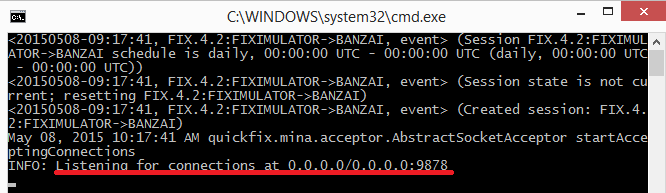
\includegraphics[scale=0.75]{figures/FIXimulator-startup.png}}
\caption{The command line logging window for the FIXimulator tool}
\label{fig:fiximulator-startup}
\end{figure}

Once the tool has been launched successfully, we can connect from kdb+ using the library. In this example the FIXimulator is acting as the acceptor, so we need to create an initiator with the \mintinline{q}{.fix.connect} function. As we can see from the console window in the previous figure, the acceptor session is \mintinline{q}{FIX.4.2:FIXIMULATOR->BANZAI}. We need to configure our initiator to have the inverse of this session id: \mintinline{q}{FIX.4.2:BANZAI->FIXIMULATOR}.

\begin{figure}[H]
\begin{qcode}
/ Build up our settings so that they can be passed in as a dictionary to the .fix.connect function.
/ FIXimulator requires that we use the FIX 4.2 specification. (remember to change the host + port to
/ be appropriate for your machine)
q) connkeys:`BeginString`SocketConnectHost`SocketConnectPort`SenderCompID`TargetCompID`DataDictionary
q) connvalues:(`FIX.4.2;`192.168.1.70;`9878;`BANZAI;`FIXIMULATOR;`$"config/spec/FIX.4.2.xml")

/ We can then open a connection.
q) .fix.connect[connkeys!connvalues]
\end{qcode}
\caption{Opening a connection to the FIXimulator tool from kdb+ using the fix engine library}
\end{figure}

If the connection has been successful, you will be able to see output in the console window and the "Client connecton status" icon at the bottom of the simulator should turn green. You should also see some output in the logs for the fix engine (which are directed to stdout by default).

\begin{figure}[H]
\centering
\fbox{
\includegraphics[scale=0.75]{figures/FIXimulator-status-bar.png}}
\caption{The FIXimulator status bar located at the bottom of the GUI}
\label{fig:fiximulator-status-bar}
\end{figure}

Once we have valid connection to the FIXimulator tool, we can click on the "Load" tab and start the
two background thread that will send IOI messages. To start the thread, scroll the slider to determine
the number of IOIs per minute and then click the "Start" button.

\begin{figure}[H]
\centering
\fbox{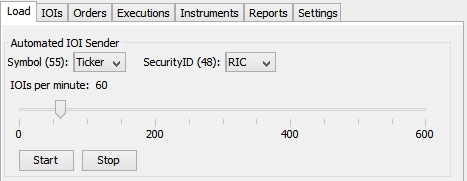
\includegraphics[scale=0.75]{figures/FIXimulator-load-tab.png}}
\caption{The "Load" tab that will allow us to send IOI messages to our kdb+ fix client}
\label{fig:fiximulator-load-tab}
\end{figure}

To view these messages in the kdb+ fix client, we need to overwrite the \mintinline{q}{.fix.onrecv}
function with our own version. For the moment, we will just write the recieved message out to the 
console.

\begin{figure}[H]
\begin{qcode}
/ We can override the onrecv function to do respond to IOIs with .fix.send, but we will just
/ write the contents of the dictionary out.
q) .fix.onrecv:{[d]
	show "--- START RECIEVED MESSAGE ---"; 
	/ We replace the numerical tags with the symbols that are human readable before printing.
	show (.fix.tags?key d)!value d;
	show "---  END RECIEVED MESSAGE  ---";}
/ An example of the message that would be recieved from the FIXimulator tool would be something
/ like this:
"--- START RECEIVED MESSAGE ---"
BeginString  | "FIX.4.2"
BodyLength   | "176"
MsgType      | ,"8"
MsgSeqNum    | "45"
SenderCompID | "FIXIMULATOR"
SendingTime  | "20150508-12:13:30.275"
TargetCompID | "BANZAI"
AvgPx        | ,"0"
ClOrdID      | "SHD2015.04.04"
CumQty       | ,"0"
ExecID       | "E1431087210278"
ExecTransType| ,"0"
LastPx       | ,"0"
LastShares   | ,"0"
OrderID      | "O1431087210281"
OrderQty     | ,"0"
OrdStatus    | ,"0"
Side         | ,"1"
Symbol       | "TESTSYM"
ExecType     | ,"0"
LeavesQty    | ,"0"
CheckSum     | "046"
"---  END RECEIVED MESSAGE  ---"
\end{qcode}
\caption{Printing the recieved IOI messages to the console}
\end{figure}

We can also send our own orders for execution. A common way of doing this would be to create a NewSingleOrder(D) message type. The function below shows how you could implement this so that
the FIXimulator will recieve the message, validate it and respond. It is also possible to create invalid messages and then send them to the simulator to see how the responses work.

\begin{figure}[H]
\begin{qcode}
q) .fix.send_new_single_order:{
	message:()!();
	message[.fix.tags.BeginString]: `FIX.4.2;
	message[.fix.tags.SenderCompID]: `BANZAI;
	message[.fix.tags.TargetCompID]: `FIXIMULATOR;
	message[.fix.tags.MsgType]: `D;
	message[.fix.tags.ClOrdID]: "SHD2015.04.04";
	message[.fix.tags.Symbol]: `TESTSYM;
	message[.fix.tags.Side]: 1;
	message[.fix.tags.HandlInst]: 2;
	message[.fix.tags.TransactTime]: .z.p;
	message[.fix.tags.OrdType]: 1;
	.fix.send[message]; }
q) .fix.send_new_single_order[]
"--- START RECEIVED MESSAGE ---"
BeginString  | "FIX.4.2"
BodyLength   | "176"
MsgType      | ,"8"
MsgSeqNum    | "45"
SenderCompID | "FIXIMULATOR"
SendingTime  | "20150508-12:13:30.275"
TargetCompID | "BANZAI"
AvgPx        | ,"0"
ClOrdID      | "SHD2015.04.04"
CumQty       | ,"0"
ExecID       | "E1431087210278"
ExecTransType| ,"0"
LastPx       | ,"0"
LastShares   | ,"0"
OrderID      | "O1431087210281"
OrderQty     | ,"0"
OrdStatus    | ,"0"
Side         | ,"1"
Symbol       | "TESTSYM"
ExecType     | ,"0"
LeavesQty    | ,"0"
CheckSum     | "046"
"---  END RECEIVED MESSAGE  ---"
\end{qcode}
\caption{Sending a new single order to the FIXimulator tool and getting an execution report back}
\end{figure}

If the message we get back is successful, then we should get a message with a type of 8 (an Execution Report) that tells us if our request has been received or not. Further messages will follow once the
tool fills the orders. You can also use the "Orders" tab of the FIXimulator tool to respond to each of
the orders manually.

\begin{figure}[H]
\centering
\fbox{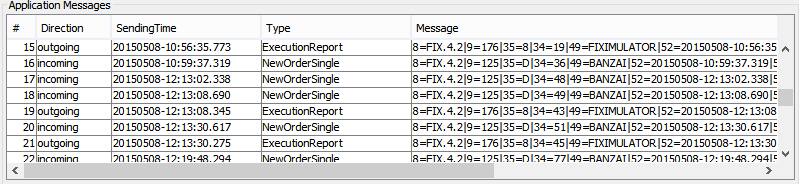
\includegraphics[scale=0.75]{figures/FIXimulator-application-messages.png}}
\caption{The application messages window in the FIXimulator tool}
\label{fig:application-messages}
\end{figure}

It is also possible to view each of the application messages as shown in figure \ref{fig:application-messages}. This will allow you to see all of the non-administrative messages
that are sent between the kdb+ fix client and the FIXimulator server. This can be useful for debugging
purposes and to ensure that all the messages have a valid format (they won't appear in this tab if they
don't follow the defined schema).

\section{Integration with TorQ}



\chapter{Shared Library API}
\section{Functions}

\subsection{.fix.setdefaults}
\label{func:setdefaults}

The .fix.setdefaults function is used to override any settings in the configuration file at runtime. It takes a dictionary of symbols -> kdb+ types and will convert the keys to uppercase before storing them in the settings. This means that the keys are case insensitive and also so that it is consistent with how the rest of the settings are stored in quickfix.

\begin{figure}[H]
\begin{qcode}
q) .fix.setdefaults[(enlist `SenderCompID)!(enlist `NewCompID)]
\end{qcode}
\caption{Replacing the default SenderCompID field with NewCompID}
\end{figure}

Any keys that are not relevant to the acceptors or initiators will be still stored in
the defaults dictionary, but ignored by the library. As long as the keys of the dictionary are a list of symbols, then this call will always succeed. 

\subsection{.fix.getdefaults}
\label{func:getdefaults}

The .fix.getdefaults functions just returns a dictionary of symbols -> symbols that contains a merged view of the configuration files and the global default set via \mintinline{q}{.fix.setdefaults}. The values that have been set using \mintinline{q}{.fix.setdefaults} take precedence over the configuration file settings.

\begin{figure}[H]
\begin{qcode}
q) .fix.getdefaults[]
APPDATADICTIONARY| config/spec/FIX.4.4.xml
BEGINSTRING      | FIX.4.4
CONNECTIONTYPE   | acceptor
DATADICTIONARY   | config/spec/FIX.4.4.xml
ENDTIME          | 23:30:00
FILELOGBACKUPPATH| logs/backup
FILELOGPATH      | logs
FILESTOREPATH    | store
HEARTBTINT       | 15
PERSISTMESSAGES  | Y
RECONNECTINTERVAL| 60
SOCKETACCEPTPORT | 7070
SOCKETNODELAY    | Y
STARTTIME        | 00:30:00
\end{qcode}
\caption{Listing the default settings from the configuration file \& those set via \mintinline{q}{.fix.setdefaults}}
\end{figure}

\subsection{.fix.listen}
\label{func:listen}

The .fix.listen function will create an acceptor that can bind to a socket and communicate with initiators. If it is passed no arguments it will take its arguments from the configuration file
and the global runtime defaults. Any arguments that are not relevant to quickfix will just be
ignored.

\begin{figure}[H]
\begin{qcode}
/ This creates an acceptor with all the default arguments.
.fix.listen[] 
/ We can also override the different options 
.fix.listen[(enlist `BeginString)!enlist `FIX.4.4]
.fix.listen[`SenderCompID`TargetCompID!`BuySideID`SellSideID]
\end{qcode}
\caption{Demonstration of how to create an acceptor using the .fix.listen function}
\end{figure}

\subsection{.fix.connect}
\label{func:connect}

The \mintinline{q}{.fix.connect} function will create an initiator that can connect to acceptors, which could be created using \mintinline{q}{.fix.listen} (section \ref{func:listen}) or be provided by a counterparty. If the \mintinline{q}{`BeginString} property is set and \mintinline{q}{`DataDictionary}
is not in the defaults, then we automatically set the \mintinline{q}{`DataDictionary},\mintinline{q}{`AppDataDictionary} to match the begin string so we can enable automatic message validation.

\begin{figure}[H]
\begin{qcode}
/ This creates an initiator with all the default arguments.
.fix.connect[]
/ We can also override the different options
.fix.connect[`BeginString`TargetCompId!`FIX.4.2`BuySideID]
\end{qcode}
\caption{Connecting to a fix adaptor using connecting to a counterparty fix adaptor}
\end{figure}

The function takes either no arguments (in which case it will pull all of its configuration from the default config file), or a dictionary of options that
should be used in place of the defaults. If the connection is not successful, the
initiator will continue to try to connect to the until.

\subsection{.fix.send}
\label{func:send}

The \mintinline{q}{.fix.send} function takes a dictionary that maps long integers to any other kdb+ type. The dictionary should contain all the correct FIX tags and a session associated with the TargetCompID and the SenderCompID should exist. The session should have been created within the same kdb+ instance using \mintinline{q}{.fix.connect} (section \ref{func:connect}) or \mintinline{q}{.fix.listen} (section \ref{func:listen}). If a session that is associated with the message doesn't exist, then a 'session error will be raised and a more detailed message will be written to stderr.

\begin{figure}[H]
\begin{qcode}
q) message:(8 35 46 ...)!(`FIX.4.4;`D;`SellerID ...)
q) .fix.send[message]
\end{qcode}
\caption{Sending a FIX message by creating a dictionary and filling it with tags.}
\end{figure}

The \mintinline{q}{.fix.send} function will use the BeginString, SenderCompID, and TargetCompID fields in order to lookup which session the message is intended for.
This means that these three fields must be set in every message dictionary. 

If the message has an invalid header or doesn't contain all the required fields, then a `config error will be raised in kdb+ and a more detailed error message will be sent to stderr. The validation is performed by the FIX engine that is recieving the message
and not locally.

\subsection{.fix.onrecv}
\label{func:onrecv}

The \mintinline{q}{.fix.onrecv} function can be defined to take a dictionary and will be called for each non-administrative message that is recieved (i.e. it won't be called for heartbeats, login, logout as these should be automatically handled by the quickfix library). It will typically be called after one of the participants in a session has used \mintinline{q}{.fix.send} (section \ref{func:send}). 

\begin{figure}[H]
\begin{qcode}
/ Defining a handler that will just print the dictionary to
/ screen. It will be called each time a non-administrative
/ message is recieved.
q) .fix.onrecv:{[dict] show dict; }
...
8 | FIX.4.4
9 | 112
35| D
34| 250
49| SellSideID
\end{qcode}
\caption{Recieving a FIX message using the .fix.onrecv handler. Each FIX field is mapped to a dictionary entry for easy consumption. }
\end{figure}

You may add any logic that you want inside the callback function to handle the dictionary, including sending response messages, disconnecting clients or storing
the data in a kdb+ database.

\subsection{.fix.getsessions}
\label{func:getsessions}

The .fix.getsessions function returns a table of all the currently running sessions within the q process and some of their configuration settings. A session corresponds
to a single acceptor or initiator that has been launched with \mintinline{q}{.fix.listen} (section \ref{func:listen}) or \mintinline{q}{.fix.connect} (section \ref{func:connect}). Sessions that are no longer
running will be removed from this table.

\begin{figure}[H]
\begin{qcode}
/ The .fix.getsessions function returns a standard kdb+ table containing the details
/ of all the active sessions.
q) .fix.getsessions[]
beginString senderCompID targetCompID sessionQualifier isInitiator ...
------------------------------------------------------------------ ...
FIX.4.4     BuySideID    SellSideID                    0           ...
FIX.4.4     SellSideID   BuySideID    SB2015050100     1           ...

/ We can query the contents of the table to extract all the sessions that are using
/ FIX 4.4 for example.
q) select senderCompID, targetCompID from .fix.getsessions[] 
		where beginString = `$"FIX.4.4"
\end{qcode}
\caption{Viewing and querying the FIX session table}
\end{figure}

\section{Enumerations}
\subsection{.fix.tags}
The .fix.tags dictionary has been built from the C++ headers in order to make building/decoding FIX messages by hand easier. To load this dictionary just load
the fixenums.q script into your session \textbf{after} loading the shared library.\\

\begin{figure}[H]
\begin{qcode}
q) .fix.tags
               | ::
BeginSeqNo     | 7
BeginString    | 8
BodyLength     | 9
CheckSum       | 10
EndSeqNo       | 16
MsgSeqNum      | 34
MsgType        | 35
...

/ We can look up which integer maps to a specific tag e.g. $\textbf{BeginString}$
q) .fix.tags.BeginString
8

/ A reverse lookup can also be performed using the find ($\textbf{?}$) 
/ operator as each integer maps to a single tag.
q) .fix.tags?8
`BeginString
\end{qcode}
\caption{Using the .fix.tags dictionary to map between the integer form \& the human readable representation}
\label{fig:tags}
\end{figure}

The \verb|fixenums.q| file has been generated by a python script located in
\verb|src/python| in the project. To create a new version of the \verb|fixenums.q| file, copy the headers from the \verb|include/quickfix| directory into the same
directory as the python script and then run \textbf{parseheaders.py}.

\subsection{.fix.values}

The values dictionary contains several nested dictionarys that contain constants that
have been defined in the standard. These constants should be used where possible in order to remain
portable. It is also possible to use these fields to "decode" the FIX messages as before using the
find operator.

\begin{qcode}
q) .fix.values.msgtype
               | ::
Heartbeat      | `0
TestRequest    | `1
ResendRequest  | `2
Reject         | `3
...
q) .fix.values.msgencoding
               | ::
ISO2022JP      | `ISO-2022-JP
EUCJP          | `EUC-JP
...
q) .fix.values.orderstatus
               | ::
New            | `0
PartiallyFilled| `1
Filled         | `2
DoneForDay     | `3
Canceled       | `4
PendingNew     | `A
\end{qcode}
